

\chapter*{Introduzione}
Innanzitutto, bisogna classificare i problemi di ottimizzazione. Diciamo che un problema di ottimizzazione può avere uno o più \textbf{decisori}, ossia delle persone o cose che prendono decisioni. I problemi con più decisori rientrano nel contesto della \textbf{Teoria dei giochi}. 
Inoltre, un'ulteriore classificazione si fa in base al numero di obiettivi, nel caso in cui vi sia un solo obiettivo parliamo di \textbf{ottimizzazione matematica} mentre, se abbiamo più obiettivi, si parla di \textbf{ottimizzazione multi-obiettivo}. Infine, nel caso di ottimizzazione matematica possiamo avere problemi \textbf{deterministici} o problemi \textbf{stocastici}. In questa trattazione ci occuperemo di problemi con un solo decisore, con un solo obiettivo e con problemi deterministici.\\
Definiamo un problema di ottimizzazione come un problema che si pone di soddisfare un obiettivo sotto certe limitazioni. Dal punto di vista matematico, ottimizzare vuol dire cercare il massimo o il minimo di una certa \textbf{funzione obiettivo} sotto certi vincoli.

Dal problema reale alla formulazione matematica si passa adottando l'approccio modellistico che prevede 5 passaggi: 
\begin{enumerate}
    \item \textbf{Analisi del problema}: definiamo l'obiettivo e le limitazioni del problema e la raccolta dei dati;
    \item \textbf{Costruzione del modello}: introduciamo le variabili, la funzione obiettivo e i vincoli;
    \item \textbf{Analisi teorica del problema}: verifichiamo l'esistenza della soluzione, la sua unicità ecc.;
    \item \textbf{Risoluzione}: individuiamo il metodo di risoluzione e avviamo l'algoritmo;
    \item \textbf{Validazione}: collaudiamo e ottimizziamo la soluzione al problema.
\end{enumerate}

Un generico problema di ottimizzazione può essere espresso nella forma:
\[\max_{x \in X} f(x) \quad \text{o} \quad \min_{x \in X} f(x)\]
dove:
\begin{itemize}
    \item \( X \subseteq \mathbb{R}^n \) è l'\textbf{insieme dei vincoli}, o \textbf{regione ammissibile}, che rappresenta l'insieme di tutti i punti che soddisfano i vincoli del problema;
    \item ogni \( x \in X \) è detto \textbf{punto ammissibile};
    \item il vettore \( x = (x_1, \ldots, x_n) \in X \) è detto \textbf{vettore delle variabili decisionali}.
\end{itemize}

Per convenzione, affronteremo sempre problemi di \textbf{minimizzazione}. \\
Infatti, ogni problema di massimo può essere ricondotto a un problema di minimo osservando che:
\[\max_{x \in X} f(x) = -\min_{x \in X} [-f(x)]\]

Un problema di ottimizzazione si definisce \textbf{inammissibile} se la regione ammissibile è vuota a causa delle restrizioni imposte, cioè, $X = \emptyset$.
Per un piccolo ripasso diremo anche che:
\begin{itemize}
    \item Un punto $x'\in X$ è detto \textbf{minimo globale} se $f(x')\leq f(x) \forall x\in X$;
    \item Un punto $x'\in X$ è detto \textbf{minimo locale} se $f(x')\leq f(x) \forall x\in I_c$ dove I è un intorno di centro c.
\end{itemize}

\chapter{Programmazione lineare continua}
Un generico problema di programmazione lineare ha sia funzione obiettivo che vincoli \textbf{lineari}, cioè, sono del tipo:
\begin{align*}
    &min(c_1x_1+...+c_nx_n) \quad \text{Funzione obiettivo}\\
    &a_{11}x_1+...+a_{1n}x_n \leq b \quad \\
    \quad\quad\quad\quad\quad\quad\quad\quad &\vdots \\
    &a_{m1}x_1+...+a_{mn}x_n \leq b \quad \text{Vincolo/i} \\
\end{align*}

I problemi di programmazione lineare devono rispettare 3 proprietà:
\begin{itemize}
    \item \textbf{Additività:} sommiamo i contributi delle variabili $c_1x_1+...+c_nx_n$;
    \item \textbf{Proporzionalità:} ogni variabile dà un contributo proporzionale a sé stessa, cioè, compare come $c_ix_i$;
    \item \textbf{Continuità:} le variabili assumono valore in R.
\end{itemize}

\section{Problemi di pianificazione della produzione}
Un problema di pianificazione della produzione si può definire a questo modo. 
Si vogliono realizzare $P_1,\dots,P_n$ prodotti, a partire da $R_1,\dots,R_m$ risorse. Ogni prodotto $P_j$ è venduto al prezzo $C_j$ ed è nota la quantità $a_{ij}$ di risorse R usate per la costruzione di $P_j$. L'obiettivo di questo problema sarà quello di massimizzare il profitto scegliendo quanto produrre di quale prodotto.
Un esempio di questo problema è il seguente. Si vogliono produrre tavoli e sedie in modo da massimizzare il profitto. Si hanno a disposizione 6 mattoni grandi e 8 mattoni piccoli e sappiamo che un tavolo è venduto a 20€ e una sedia a 15 €. 
\begin{table}[H]
    \centering
    \begin{tabular}{|c|c|c|}
        \hline
        & \textbf{Sedia} & \textbf{Tavolo} \\
        \hline
        \textbf{grandi} & 1 & 2 \\
        \hline
        \textbf{piccoli} & 2 & 2 \\
        \hline
    \end{tabular}
    \caption{Quantità di mattoncini per prodotto}
    \label{tab:mobili_dimensione}
\end{table}

Possiamo adesso costruire il modello tramite delle variabili per risolvere il problema. Per costruire il modello di programmazione lineare occorre:
\begin{enumerate}
    \item Definire il tipo di problema;
    \item Trovare le variabili;
    \item Costruire la funzione obiettivo;
    \item Determinazione dei vincoli.
\end{enumerate}

Avremo bisogno delle variabili $x_1$ per il numero di sedie e $x_2$ per il numero di tavoli. Di conseguenza, la nostra funzione obiettivo da massimizzare è $15x_1+20x_2$.
Per quanto riguarda i vincoli, invece, avremo le seguenti disequazioni:
\begin{equation*}
    \begin{cases}
        x_1 + 2x_2 \le 6 & (\text{Vincolo Mattoni Grandi}) \\
        2x_1 + 2x_2 \le 8 & (\text{Vincolo Mattoni Piccoli}) \\
        x_1 \ge 0, x_2 \ge 0 & (\text{Non-Negatività})
    \end{cases}
\end{equation*}

\subsection{Risoluzione grafica}
Un problema di programmazione lineare si può risolvere mediante \textbf{risoluzione grafica} che si può applicare solo in caso di problemi con 2 variabili. Questa soluzione si basa sulla rappresentazione grafica della funzione obiettivo e dei vincoli. Vediamo come questo si applica al problema della produzione che abbiamo citato prima. 
I due vincoli rappresentano due semi-piani che possiamo rappresentare disegnando la \textbf{retta associata} \footnote{Ci basterà scegliere due punti che rispettano l'equazione.} e segnando il piano indicato dalla disequazione. \footnote{Possiamo effettuare la prova con dei punti sopra o sotto la retta per vedere quale piano è associato.} Fatto ciò, l'intersezione dei due semipiani rappresenterà la così detta \textbf{regione ammissibile} che rappresenterà tutti i punti validi che rispettano i vincoli.  Disegniamo la retta della funzione obiettivo con guadagno minimo che, in questo caso sarà $(0,0)$, e spostiamo la retta in direzione del gradiente\footnote{Il gradiente è il vettore dei coefficienti della retta} per massimizzare il prodotto.\footnote{Se dobbiamo minimizzare, operiamo al contrario}  

\begin{figure}[H]
    \centering
    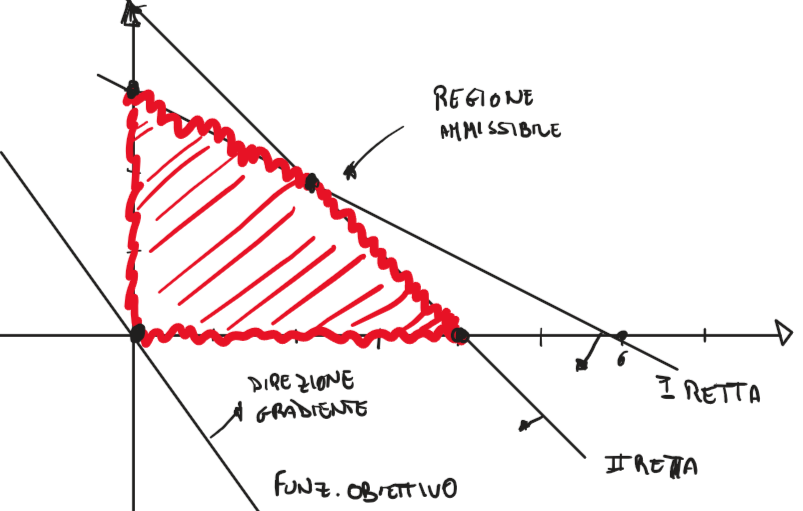
\includegraphics[width=0.55\linewidth]{Images/risoluzione_grafica.png}
    \caption{Risoluzione grafica del problema}
    \label{fig:risoluzione_grafica}
\end{figure}

Un problema di programmazione lineare può avere:
\begin{enumerate}
    \item Una sola soluzione su un solo vertice;
    \item Infinite soluzioni se si abbraccia un lato della regione ammissibile (delle quali almeno un vertice. 
\end{enumerate}
Inoltre, può non avere soluzioni se:
\begin{enumerate}
    \item La regione ammissibile è vuota;
    \item La funzione obiettivo non è limitata.
\end{enumerate}

Caso particolare: la regione ammissibile non è limitata. In questo caso avremo infinite soluzione ottime senza avere vertici.

\section{Geometria della programmazione lineare}

Dati \( v_1, \ldots, v_n \in \mathbb{R}^n \), la loro \textbf{combinazione lineare} è il vettore:
\[
a_1v_1 + a_2v_2 + \ldots + a_nv_n, 
\quad \text{con } a_i \in \mathbb{R}.
\]

Dati i vettori \( v_1, \ldots, v_m \in \mathbb{R}^n \), la \textbf{combinazione convessa} è il vettore:
\[
v = a_1v_1 + a_2v_2 + \ldots + a_mv_m,
\quad a_i \geq 0 \; \forall i = 1, \ldots, m,
\quad \sum_{i=1}^{m} a_i = 1.
\]

Dati \( v_1, v_2 \in \mathbb{R}^n \), si dice \textbf{segmento} l'insieme di tutte le combinazioni convesse di \( v_1 \) e \( v_2 \).\footnote{In pratica, tutti gli infiniti punti che compongono un segmento.}

Guardiamo un esempio con:
\[
v_1 = (1, 2), \quad v_2 = (3, 4).
\]

\begin{figure}[H]
    \centering
    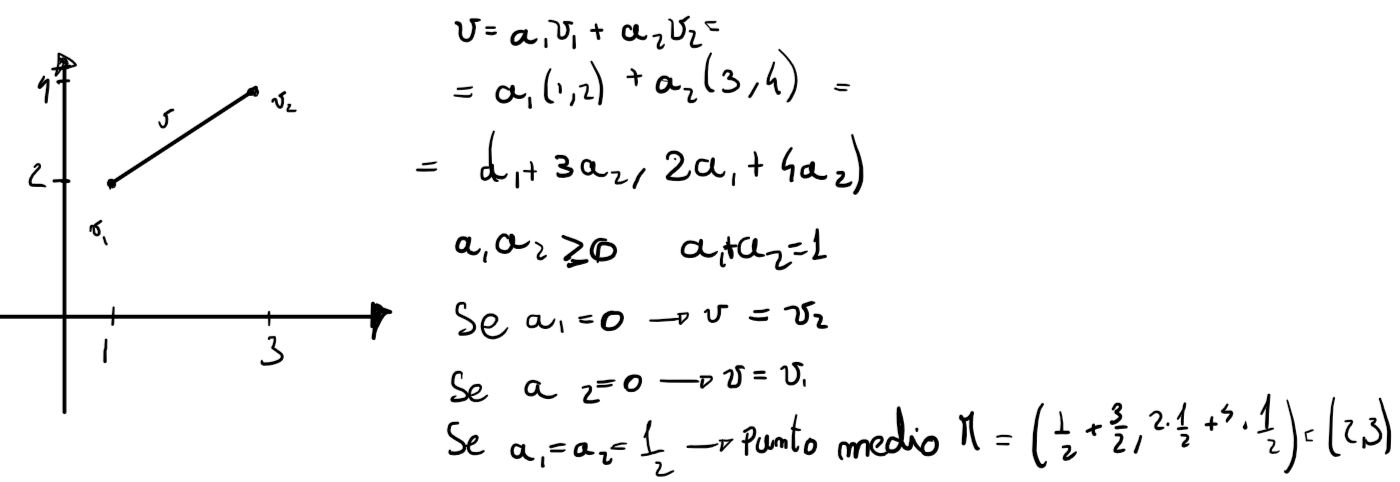
\includegraphics[width=1\linewidth]{Images/segmento.png}
    \label{fig:segmento}
\end{figure}

Allo stesso modo definiamo \textbf{combinazione convessa stretta} il vettore:
\[
v = a_1v_1 + (1 - a_1)v_2, 
\quad a_1 \in (0,1).
\]

Un insieme \( X \subseteq \mathbb{R}^n \) è detto \textbf{convesso} se 
\[
\forall\, x, y \in X, \quad \forall\, \lambda \in [0,1], \quad 
z = \lambda x + (1 - \lambda)y \in X.
\]
In altre parole, ogni segmento che congiunge due punti appartenenti a \( X \) è interamente contenuto in \( X \).

\vspace{1em}

Diamo alcune definizioni:

\begin{itemize}
    \item Si dice \textbf{iperpiano} l'insieme dei punti che sono soluzioni dell'equazione:
    \[
    a_1x_1 + a_2x_2 + \ldots + a_nx_n = b
    \]
    oppure, in forma compatta:
    \[
    a^T x = b,
    \quad (a_1, \ldots, a_n) \in \mathbb{R}^n, 
    \quad (a_1, \ldots, a_n) \neq (0, \ldots, 0), 
    \quad b \in \mathbb{R}.
    \]
    Questo generalizza il concetto di retta.

    \item Si dice \textbf{semispazio} l'insieme dei punti che sono soluzioni della disequazione:
    \[
    a_1x_1 + a_2x_2 + \ldots + a_nx_n \leq b.
    \]

    \item Si dice \textbf{poliedro} l'intersezione di un numero finito di iperpiani e semispazi.  
    Per definizione, ogni poliedro è un insieme convesso.
\end{itemize}

\vspace{1em}

Possiamo quindi riscrivere i problemi di programmazione lineare in questo modo:
\[
\begin{aligned}
&\max/\min \quad (c_1x_1 + c_2x_2 + \ldots + c_nx_n) \\
&\text{soggetto a:} \\
&a_{11}x_1 + a_{12}x_2 + \ldots + a_{1n}x_n \leq b_1 \\
&a_{21}x_1 + a_{22}x_2 + \ldots + a_{2n}x_n \leq b_2 \\
&\vdots \\
&a_{m1}x_1 + a_{m2}x_2 + \ldots + a_{mn}x_n \leq b_m
\end{aligned}
\]

L'insieme dei vincoli, da un punto di vista algebrico, è un sistema di equazioni e disequazioni lineari in \( n \) variabili.  
Un'equazione lineare rappresenta un iperpiano, mentre una disequazione lineare rappresenta un semispazio.  
La \textbf{regione ammissibile} è quindi l'intersezione di un numero finito di iperpiani e semispazi, cioè un poliedro.

Essendo la regione ammissibile un poliedro, essa è anche un insieme convesso.  
Ne consegue che il problema di programmazione lineare è un \textbf{problema convesso}.

\vspace{1em}

Usando le definizioni precedenti, possiamo definire meglio il concetto di vertice:  
dato un poliedro \( P \), si dice \textbf{vertice} un punto di \( P \) che non può essere scritto come combinazione convessa stretta di altri punti di \( P \).  
In altre parole, un vertice è un punto esterno dei segmenti che formano \( P \), e non un punto interno.  
Un poliedro ha vertici se e solo se non contiene rette.

\section{Teorema fondamentale della programmazione lineare}

Sia dato un poliedro 
\[
P = \{\, x \in \mathbb{R}^n \mid A x \leq b \,\}
\]
con \( A \in \mathbb{R}^{m \times n} \) e \( b \in \mathbb{R}^m \), tale che \( P \neq \emptyset \) e \( P \) non contenga rette.  
Sia dato il problema di programmazione lineare:
\[
\min (c^T x) \quad \text{soggetto a } x \in P
\]
allora la funzione obiettivo o non è limitata inferiormente, oppure il problema ammette almeno un ottimo finito in uno dei vertici di \( P \).

\vspace{1em}

In parole semplici, questo teorema ci dice che, se esiste un ottimo, esso si trova in uno dei vertici del poliedro \( P \).  
Grazie a una proprietà di tipo \textit{greedy}, sappiamo inoltre che un vertice è ottimo se e solo se nessuno dei suoi vertici adiacenti fornisce un valore migliore della funzione obiettivo.


\section{Algebra della Programmazione Lineare}

Adesso che abbiamo dato alcune definizioni, possiamo portare tutta la geometria in termini vettoriali.  
Si chiama \textbf{forma standard} di un problema di programmazione lineare il problema:

\[
\begin{aligned}
&\min(c_1x_1 + c_2x_2 + \ldots + c_nx_n) \\
\\
\text{soggetto a:} \quad 
&a_{11}x_1 + a_{12}x_2 + \ldots + a_{1n}x_n \leq b_1 \\
&a_{21}x_1 + a_{22}x_2 + \ldots + a_{2n}x_n \leq b_2 \\
&\vdots \\
&a_{m1}x_1 + a_{m2}x_2 + \ldots + a_{mn}x_n \leq b_m \\
&b_1, \ldots, b_m \geq 0
\end{aligned}
\]

Che soddisfi i requisiti:
\begin{enumerate}
    \item Problema di minimo;
    \item Tutti i vincoli sono di uguaglianza;
    \item Tutte le variabili non devono essere negative;
    \item I termini noti non devono essere negativi.
\end{enumerate}


È possibile ricondurre tutti i problemi di programmazione lineare in forma standard seguendo le seguenti procedure:

\begin{itemize}
    \item \textbf{Problema di massimo}:  
    Possiamo ricondurre i problemi di massimo a problemi di minimo cambiando:
    \[
    \max(c_1x_1 + \ldots + c_nx_n) 
    \quad \longrightarrow \quad 
    -\min(-c_1x_1 - \ldots - c_nx_n)
    \]
    Ricordiamo che modificheremo solo la funzione obiettivo e non i vincoli.
    
    \item \textbf{Vincolo minore o uguale}:  
    Introduciamo una variabile di \textbf{scarto (slack)} \( x_{n+1} \ge 0 \), ottenendo:
    \[
    \sum_{j=1}^n a_{ij}x_j + x_{n+1} = b_i
    \]
    Esempio:
    \[
    3x_1 + 5x_2 - x_3 \le 8 
    \quad \xrightarrow{\text{aggiungo slack}} \quad
    3x_1 + 5x_2 - x_3 + x_4 = 8, \quad x_4 \ge 0
    \]

    \item \textbf{Vincolo maggiore o uguale}:  
    Introduciamo una variabile di \textbf{surplus} \( x_{n+1} \ge 0 \), ottenendo:
    \[
    \sum_{j=1}^n a_{ij}x_j - x_{n+1} = b_i
    \]
    Esempio:
    \[
    3x_1 + 5x_2 - x_3 \ge 8 
    \quad \xrightarrow{\text{aggiungo surplus}} \quad
    3x_1 + 5x_2 - x_3 - x_4 = 8, \quad x_4 \ge 0
    \]

    \item \textbf{Vincolo per variabile} \( \le 0 \):  
    Introduciamo una nuova variabile \( x'_j \ge 0 \) e poniamo \( x'_j = -x_j \).  
    Esempio:
    \[
    \begin{aligned}
    &\min(x_1 - x_2) \\
    &2x_1 + x_2 \le 6 \\
    &3x_1 + x_2 \le 8 \\
    &x_1 \ge 0, \quad x_2 \le 0
    \end{aligned}
    \]
    Ponendo \( x'_2 = -x_2 \ge 0 \), otteniamo:
    \[
    \begin{aligned}
    &\min(x_1 + x'_2) \\
    &2x_1 - x'_2 \le 6 \\
    &3x_1 - x'_2 \le 8 \\
    &x_1 \ge 0, \quad x'_2 \ge 0
    \end{aligned}
    \]

    \item \textbf{Variabile priva di segno}:  
    Se una variabile \( x_j \) non ha vincoli di segno, introduciamo due variabili non negative \( x'_j, x''_j \ge 0 \) e poniamo:
    \[
    x_j = x'_j - x''_j
    \]
    Esempio:
    \[
    \begin{aligned}
    &\min(3x_1 + 2x_2) \\
    &x_1 + 4x_2 = 6 \\
    &x_1 + 3x_2 = 8 \\
    &x_1 \ge 0
    \end{aligned}
    \]
    Poniamo \( x_2 = x'_2 - x''_2, \; x'_2, x''_2 \ge 0 \), ottenendo:
    \[
    \begin{aligned}
    &\min(3x_1 + 2(x'_2 - x''_2)) \\
    &x_1 + 4(x'_2 - x''_2) = 6 \\
    &x_1 + 3(x'_2 - x''_2) = 8 \\
    &x_1 \ge 0, \quad x'_2, x''_2 \ge 0
    \end{aligned}
    \]
\end{itemize}

\chapter{Metodo del Simplesso}
Il metodo del simplesso parte dall'idea di verificare un vertice e, se questo non è ottimale, ci spostiamo su un altro vertice adiacente sulla base di alcuni criteri che vedremo tra poco. I problemi di programmazione lineare, come già detto, hanno una funzione obiettivo lineare e l'insieme dei vincoli convesso. Questi sono problemi di ottimizzazione convessa, per cui, gli ottimi locali sono anche ottimi globali.

La forma standard è $min(c^Tx) \quad Ax = b \quad x\geq 0 \quad A \in R^{m * n}$, inoltre, il rango della matrice A deve essere uguale a m e $m<n$. Questo perché:
\begin{itemize}
    \item Se  $m = n$, la matrice è una matrice quadrata $n\times n$ e, $rango(A)=n$ per cui la matrice sarebbe non invertibile e il sistema avrebbe una sola soluzione.
    \item Se  $m > n$, vuol dire che abbiamo dei vincoli ridondanti poiché abbiamo più righe che colonne, cioè, alcune righe si possono eliminare senza alterare la struttura del poliedro. Dunque, si ritorna al caso m < n. 
\end{itemize}
Data una matrice $A \in \mathbb{R}^{m \times n}$, con $n \ge m$ e rango massimo, ovvero $\text{rango}(A) = m$.
Si definisce \textbf{matrice di base} $B$ una qualsiasi sottomatrice quadrata $B \in \mathbb{R}^{m \times m}$ ottenuta da $A$ selezionando $m$ delle sue $n$ colonne, tali che queste $m$ colonne siano linearmente indipendenti.

L'ipotesi $\text{rango}(A) = m$ garantisce l'esistenza di almeno una tale sottomatrice $B$.\footnote{Il rango di una matrice ci dice il numero di vettori linearmente indipendenti.}
Inoltre, poiché $B$ è una matrice $m \times m$ con $m$ colonne linearmente indipendenti, $B$ è \textbf{non singolare} (o invertibile), ovvero $\det(B) \neq 0$.
L'implicazione può essere scritta come:
$$
\text{rango}(A) = m \implies \exists B: \det(B) \neq 0
$$
\begin{figure}[H]
    \centering
    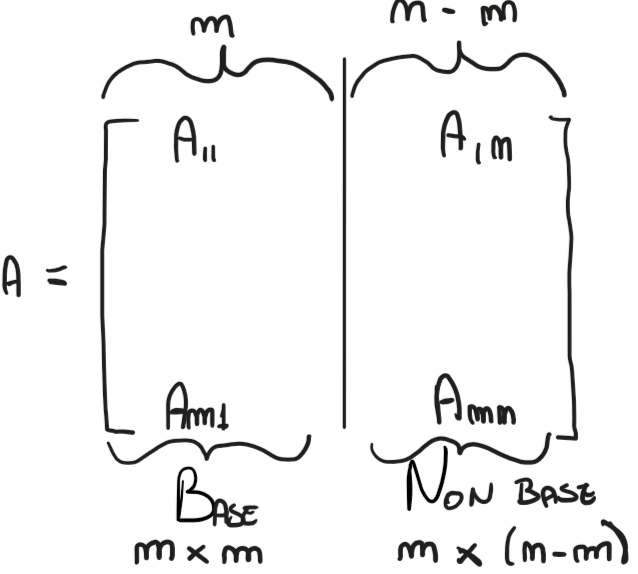
\includegraphics[width=0.33\linewidth]{Images/matrice_base_generica.png}
\end{figure}

Facciamo un esempio concreto di cosa vuol dire:
\begin{align*}
    x_1 - x_2    &\leq 2   && \implies \quad & x_1 - x_2 + x_3 \phantom{+x_4 +x_5} &= 2 \\
   2x_1 + x_2    &\leq 4   && \implies \quad & 2x_1 + x_2 \phantom{+x_3} + x_4 \phantom{+x_5} &= 4 \\
  -3x_1 + 2x_2   &\leq 6   && \implies \quad & -3x_1 + 2x_2 \phantom{+x_3 +x_4} + x_5 &= 6 \\
    x_1, x_2     &\geq 0   && \implies \quad & x_j \geq 0 \quad \forall j&=1, \dots, 5
\end{align*}
La matrice associata a questo sistema sarà:
\begin{figure}[H]
    \centering
    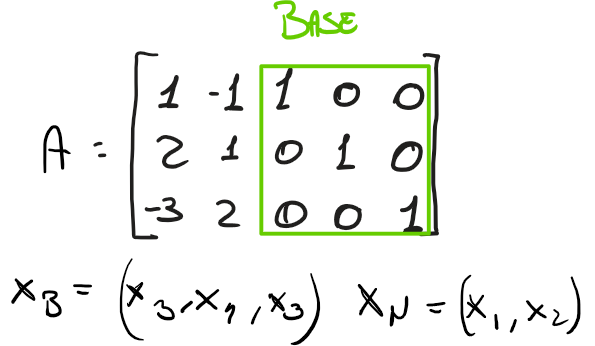
\includegraphics[width=0.45\linewidth]{Images/esempio_base.png}
\end{figure}
Avendo: 
\[x_3 = 2-x_1+x_2 \quad
x_4 = 4-2x_1-x_2 \quad
x_5 = 6+3x_1-2x_2\]
E ponendo $x_1=x_2 = 0$, cioè le variabili fuori dalla base, si troverà il vertice (0, 0, 2, 4, 6) che sarà detto \textbf{soluzione di base}. Per essere più precisi, si dice soluzione di base la soluzione del sistema $Ax = b \leftrightarrow \quad Bx_b + Nx_n = b \quad \text{con } x_b = B^{-1}b\quad x_n = 0$.

In altre parole, una soluzione di base è soluzione del sistema che si ottiene scrivendo le variabili di base in funzione di quelle fuori dalla base e ponendo uguali a zero le componenti non di base. 

Una soluzione di base si dice \textbf{ammissibile (SBA)} se le componenti di base $B^{-1} b \geq 0$. 

Una soluzione di base si dice \textbf{degenere} se ha una delle componenti di base uguale a 0. 
\\
\textbf{Teorema}\\
Dato $P = \{x\in R^n: Ax = b, x\geq 0\}, x' \in P$ è un vertice $\leftrightarrow$ è SBA. 

Il Teorema fondamentale della programmazione lineare suggerisce di cercare un vertice ottimo mentre questo teorema chiarisce che bisogna cercare una \textbf{soluzione di base ammissibile ottima}.\footnote{Questa corrisponderà ad un vertice.}

Il numero massimo di soluzioni di base ammissibili è legato al numero massimo di sottomatrici $m \times m$ estraibili da A che è una matrice $m \times n$. Quindi ci sono al più $\binom{n}{m}$ basi, fra queste ci sono anche delle sottomatrici non invertibili e sottomatrici che danno soluzioni di base non ammissibili.  Quindi $\binom{n}{m}$ è abbondantemente > del numero di soluzioni di base ammissibile. 

\section{Forma Canonica}
Un problema in forma standard può sempre essere posto nella forma canonica, secondo la quale la matrice di base B è la matrice identità e tutte le variabili di base possono essere espresse in funzione delle variabili fuori base.


Si dice \textbf{forma canonica} di un problema di programmazione lineare, il sistema dei vincoli espressi nel seguente modo:

\begin{figure}[H]
    \centering
    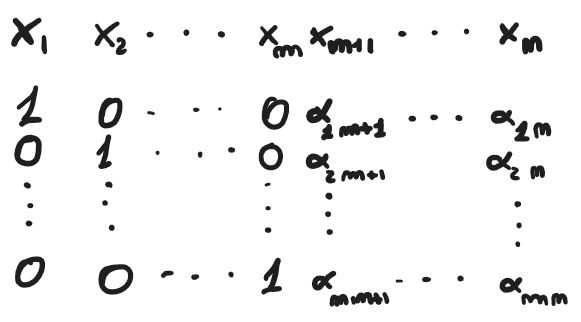
\includegraphics[width=0.5\linewidth]{Images/matrice_base_canonica.png}
\end{figure}

dove $x_1, \dots, x_m$ sono le variabili di base e $x_{m+1}, \dots, x_n$ 
sono le variabili fuori base. Ogni variabile di base è scritta in 
termini delle variabili fuori base. La soluzione di base è
\[
x_1 = \beta_1, \dots, x_m = \beta_m, x_{m+1} = 0, \dots, x_n = 0.
\]

Grazie alla forma canonica, è possibile esprimere le variabili di base in funzione di quelle non di base a questo modo:
\begin{align*}
    x_1 &= \beta_1 - \sum_{j=m+1}^{n} \alpha_{1j}x_j \\
    &\vdots \\
    x_m &= \beta_m - \sum_{j=m+1}^{n} \alpha_{mj}x_j,
\end{align*}
Possiamo anche sostituire ciò alla funzione obiettivo per cui avremo che 
\[z=  c^Tx=c_1x_1+\dots+c_mx_m+c_{m+1}x_{m+1}+\dots+c_nx_n\]
E, grazie a varie sostituzioni,\footnote{Dimostrazioni che si possono vedere dal PDF della prof.} si può arrivare a:
\[z=z_0+\sum_{j=m+1}^n(c_j-z_j)x_j \quad z_j=\sum_{j=1}^m\alpha_{ij}c_j\]
Si dice costo ridotto di una variabile $x_j$ la quantità  $r_j = c_j - Z_j \quad \forall j = 1,\dots, n$.\\
\textbf{Condizione di ottimalità}\\
Se $c_j - z_j \geq 0 \quad\quad \forall j = m+1, \dots, n $allora la funzione di base ammissibile corrente è ottima. Possiamo tradurre il tutto in, se i costi ridotti delle variabili fuori base sono $\geq 0$ allora abbiamo trovato l'ottimo.

Se il test di ottimalità non è valido, vuol dire che il vertice corrente non è ottimo e, dunque, si deve visitare un vertice adiacente e questo equivale a passare dalla base B corrente ad una base B' adiacente che differisce da B solo per una colonna.
\section{Operazioni di Pivot}
Se la soluzione di base non soddisfa il test di ottimalità, occorre visitare un'altra base. L'operazione di \textbf{pivot} serve per passare da una soluzione di base ad un'altra, sostituendo una variabile di base $x_r$ con una non di base $x_s$.\\

\begin{tabular}{| c c c c c c c c c c | c |}
\hline
% Riga d'intestazione
$x_1$ & $\dots$ & $x_r$ & $\dots$ & $x_m$ & $x_{m+1}$ & $\dots$ & $x_s$ & $\dots$ & $x_n$ & \\
\hline
% Riga 1
$1$ & $\dots$ & $0$ & $\dots$ & $0$ & $\alpha_{1,m+1}$ & $\dots$ & $\alpha_{1s}$ & $\dots$ & $\alpha_{1n}$ & $\beta_1$ \\
% Riga 2
$0$ & $\dots$ & $0$ & $\dots$ & $0$ & $\alpha_{2,m+1}$ & $\dots$ & $\alpha_{2s}$ & $\dots$ & $\alpha_{2n}$ & $\beta_2$ \\
% Riga di punti 1 (come da immagine)
$\cdot$ & $\dots$ & $\cdot$ & $\dots$ & $\cdot$ & $\cdot$ & $\dots$ & $\cdot$ & $\dots$ & $\cdot$ & $\cdot$ \\
% Riga 'r'
$0$ & $\dots$ & $1$ & $\dots$ & $\cdot$ & $\cdot$ & $\dots$ & $\alpha_{rs}$ & $\dots$ & $\cdot$ & $\cdot$ \\
% Riga di punti 2 (come da immagine)
$\cdot$ & $\dots$ & $\cdot$ & $\dots$ & $\cdot$ & $\cdot$ & $\dots$ & $\cdot$ & $\dots$ & $\cdot$ & $\cdot$ \\
% Riga 'm'
$0$ & $\dots$ & $0$ & $\dots$ & $1$ & $\alpha_{m,m+1}$ & $\dots$ & $\alpha_{ms}$ & $\dots$ & $\alpha_{mn}$ & $\beta_m$ \\
\hline
\end{tabular}
\\
\\
Per far uscire dalla base $x_r$ e per fare entrare $x_s$, innanzitutto definiamo come \textbf{perno o pivot} il valore $\alpha_{rs}\neq 0$. Dopodiché, quello che vogliamo ottenere è che $\alpha_{rs}=1$ e che tutti gli altri elementi della colonna siano $=0$. Per fare ciò, abbiamo a disposizione due trasformazioni:
\begin{enumerate}
    \item Possiamo dividere la riga del perno per un valore in maniera tale che $\alpha_{rs}=1$.
    \item Ad ogni riga possiamo sottrarre la riga del perno appena trasformata, anche moltiplicata per una costante se necessario, per annullare gli elementi di tutta la colonna. 
\end{enumerate}

\section{Criterio di entrata}
Poiché risulta che:
\[z=z_0+\sum_{j=m+1}^n(c_j-z_j)x_j\]
il valore della funzione obiettivo migliora, cioè, diminuisce dato che trattiamo problemi di minimo se 
\[\exists j, m+1\leq j\leq n:c_j-z_j<0\]
Si sceglie la variabile $x_s$ che localmente fa diminuire più rapidamente la funzione obiettivo, cioè si sceglie l'indice s per cui $c_s-z_s=min_j(c_j-z_j)$. La variabile che entra in base passa da zero ad un valore positivo che riduce il costo totale.
\section{Criterio di uscita}
Una volta scelta la variabile $x_s$ che dovrà entrare in base, la variabile uscente viene individuata in modo da rimanere nella regione ammissibile. Esce dalla base $x_r$ per cui il rapporto $\frac{\beta_r}{x_{rs}}$ è minimo e $x_s$ entra con valore $\frac{\beta_r}{\alpha_{rs}}$.\footnote{Il fatto che "entri con quel valore" sta ad indicare il fatto che il prossimo vertice avrà la coordinata $x_s=\frac{\beta_r}{\alpha_{rs}}$.}
\section{Criterio di Illimitatezza}
Se, durante l'algoritmo del simplesso, esiste un indice $s$ di una variabile non in base $x_s$ tale che:
\begin{enumerate}
    \item Il suo costo ridotto è negativo, cioè $c_s-z_s<0$.
    \item Tutti gli elementi della sua colonna sono minori o uguali a zero.
\end{enumerate}
Allora il problema di programmazione lineare è illimitato inferiormente.

\section{Forma tabellare}
Per semplificare il problema di programmazione lineare, utilizziamo una forma tabellare. Sia dato il problema
\[min(c^Tx) \quad Ax= b \quad x\geq 0\]
Introduciamo una variabile z e poniamo $z=c^Tx$ da cui deriva il nuovo vincolo per cui $-z+c^Tx = 0$, rendendo il problema 
\[min(z) \quad Ax=b \quad -z+c^Tx=0 \quad x\geq0\]
Che, in forma tabellare diventa così
\begin{figure}[H]
    \centering
    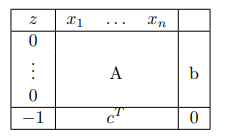
\includegraphics[width=0.3\linewidth]{Images/tabella_con_vincoli.png}
\end{figure}
Considerando che -1 è il coefficiente di z e $c^T$ sono i coefficienti di base. Scegliendo una base, la tabella cambia e abbiamo:
\begin{figure}[H]
    \centering
    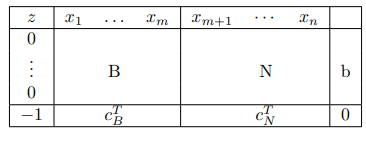
\includegraphics[width=0.5\linewidth]{Images/tabella_con_base.png}
\end{figure}
Poiché B è invertibile, abbiamo che $x_b=B^{-1}b-B^{-1}Nx_N$ e, sostituendo nel problema principale, abbiamo
\[min(z)\quad x_B+B^{-1}Nx_N=B^{-1}b \quad -z+(c^T_N-c^T_BB^{-1}N)x_N=-c^T_BB^{-1}b \quad x_B \geq 0 \quad x_N \geq 0\]
\begin{figure}[H]
    \centering
    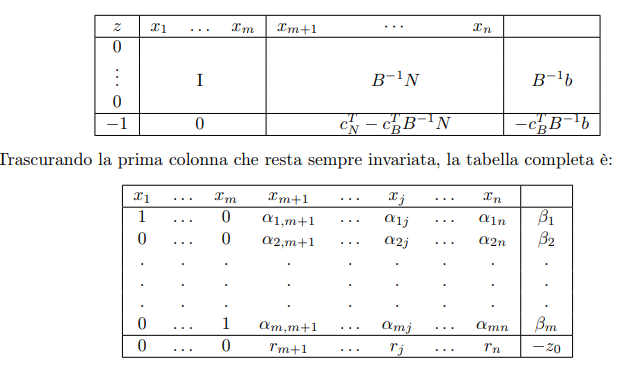
\includegraphics[width=0.8\linewidth]{Images/tabella_finale_base.png}
\end{figure}
In questa tabella:
\begin{itemize}
    \item l'ultima colonna dà il valore delle variabili di base e il valore $-z_0=-c^T_BB^{-1}b$ è l'opposto del valore corrente della funzione obiettivo.
    \item L'ultima riga è la riga dei costi ridotti.
    \item Le variabili di base corrispondono alla matrice di base che è una matrice identità $m\times m$.
\end{itemize}


\section{Algoritmo per il metodo del simplesso}
Per quanto riguarda l'applicazione pratica del metodo del simplesso, descriviamo i seguenti passi:
\begin{enumerate}
    \item Si trovi una base B che generi una soluzione ammissibile di base.
    \item Se $r_j\geq 0, \forall j$, allora possiamo fermarci e la soluzione ammissibile di base corretta è ottima. Altrimenti, si sceglie una colonna per fare entrare un'altra variabile in base tramite il criterio di entrata.
    \item Se $a_{is}\leq 0, i=1,\dots,m$, allora possiamo fermarci e il problema è illimitato. Altrimenti si calcolano i rapporti e si scelga la variabile uscente tramite il criterio di uscita.
    \item Si aggiorni la tabella e si ricominci dall'elemento (r,s) e si torni al passo 2. 
\end{enumerate}

\section{Esempio metodo del simplesso}
Vediamo adesso di risolvere un esercizio. Supponiamo di avere il seguente di programmazione lineare:
\[max(120x_1+100x_2)\quad 2x_1+2x_2\leq8 \quad 5x_1+3x_2\leq15\quad x_1,x_2\geq0\]
Portiamolo alla forma standard
\[min(-120x_1-100x_2)\quad 2x_1+2x_2+x_3=8 \quad5x_1+3x_2+x_4=15 \quad x_i\geq 0 \forall i = 1\dots4 \]
Vediamo la matrice in questo problema:
\begin{figure}[H]
    \centering
    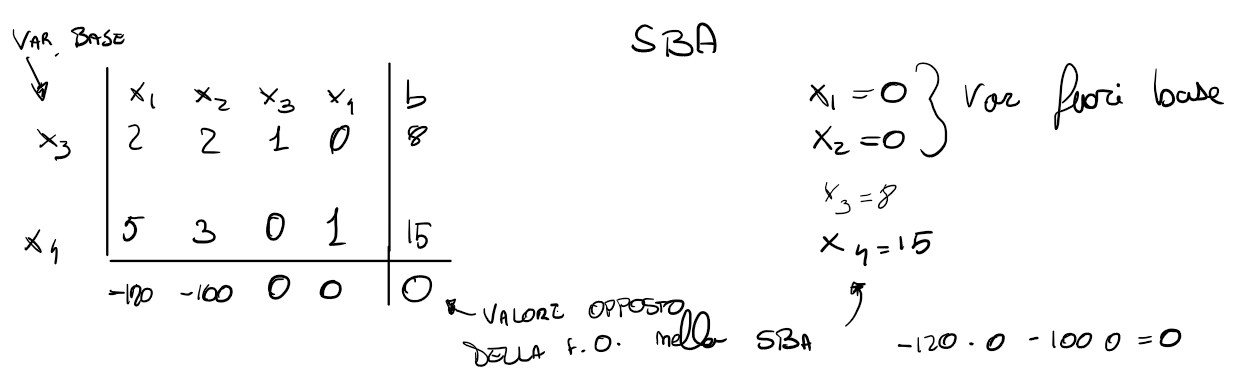
\includegraphics[width=1\linewidth]{Images//esempio_simplesso/matrice_1_simplesso.png}
\end{figure}
Nell'ultima riga sono stati inseriti i costi ridotti delle variabili fuori base come i coefficienti iniziali del problema e i costi ridotti delle variabili in base come 0. Questa cosa funziona solo nel caso in cui abbiamo solo vincoli di minore uguale.
Continuando l'esercizio, vediamo che abbiamo costi negativi nell'ultima riga, per cui abbiamo bisogno di sceglierne uno per che, per regola di base, prenderemo quello con l'indice più piccolo. In questo caso prenderemo $x_1$ che dovrà \textbf{entrare in base}.
Adesso non ci resta che capire chi deve uscire dalla base, e ciò si calcola tramite il criterio di uscita, per cui:
\[min(\frac{8}{2},\frac{15}{5})=min(4,3) = 3 \quad \text{Il primo valore ci indica $x_3$ e il secondo $x_4$}\]

Per cui, essendo 3 il più piccolo, esce dalla base $x_4$. Scegliamo come \textbf{pivot} o \textbf{perno} il valore dell'incrocio tra la riga uscente e la colonna entrante. Dopodiché, per far entrare in base $x_1$, effettuiamo delle operazioni \textbf{pivotali} e avremo:
\begin{figure}[H]
    \centering
    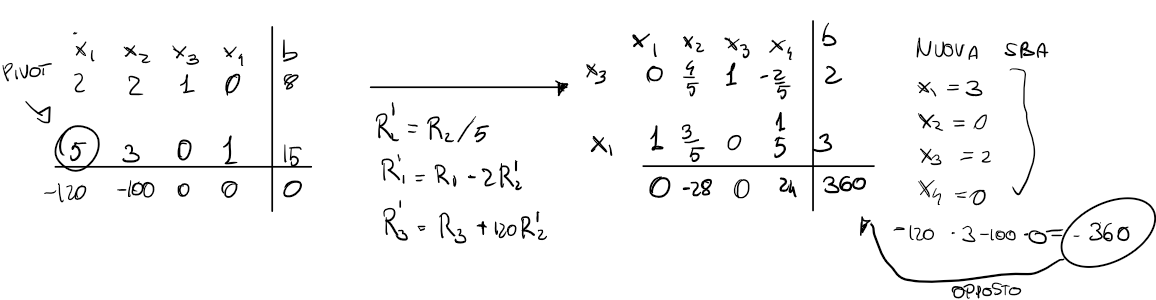
\includegraphics[width=1\linewidth]{Images//esempio_simplesso/matrice_2_esempio.png}
\end{figure}
Ancora troviamo tra i costi ridotti un valore negativo, per cui, continuiamo con l'algoritmo e facciamo entrare $x_2$ e vediamo chi fare uscire:
\[min(\frac{2}{\frac{4}{5}},\frac{3}{\frac{3}{5}})=min(\frac{5}{2},\frac{5}{3} ) = \frac{5}{2}\]
Per cui esce dalla base $x_3$ ed entra in base $x_2$.
\begin{figure}[H]
    \centering
    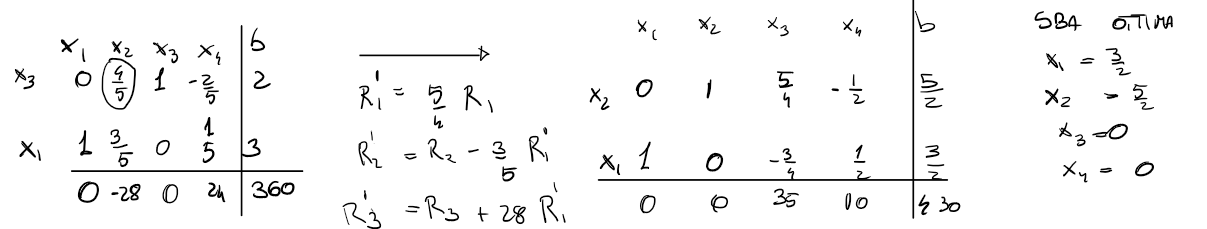
\includegraphics[width=1\linewidth]{Images//esempio_simplesso/matrice_3_esempio.png}
\end{figure}
Che è soluzione ottima del problema di minimo. Se vogliamo guardare il grafico della funzione troveremo una cosa del genere:
\begin{figure}[H]
    \centering
    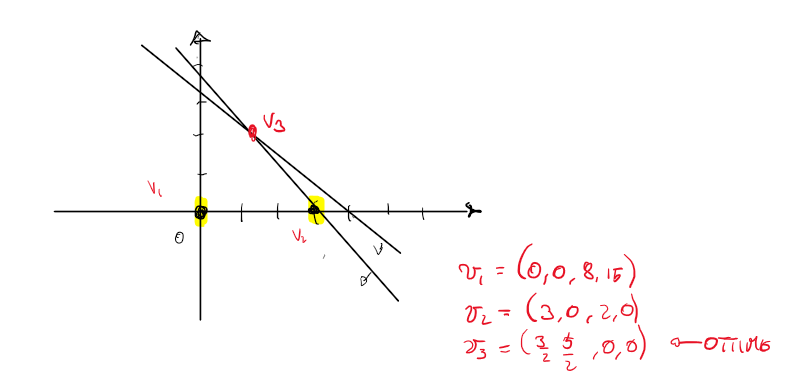
\includegraphics[width=1\linewidth]{Images//esempio_simplesso/grafico_esempio.png}
\end{figure}

\section{Convergenze del metodo, Unicità e Regola di Bland}
Il \textbf{Teorema di convergenza del metodo} stabilisce che se durante l'esecuzione del algoritmo si visitano solo soluzioni di base ammissibili non degenere, allora verranno prodotte una sequenza di basi ammissibili senza ripetizioni e, dopo un numero finito di passi, il metodo converge alla soluzione ottima o indica che il problema non è limitato inferiormente.

Una volta visitata una soluzione degenere, cioè, una soluzione per cui una variabile $x_b$ di base ha valore 0, allora si può rimanere bloccati in un vertice per un numero variabile di volte. Per evitare che ciò accada si può applicare la regola di Bland.

La \textbf{regola di Bland} stabilisce che, in caso di indecisione nel caso del criterio di entrata o di uscita\footnote{Ad esempio se per il criterio di entrata abbiamo più valori negativi o nel criterio di uscita abbiamo due valori minimi.} è opportuno scegliere la variabile che ha indice inferiore nella matrice considerata.
\begin{figure}[H]
    \centering
    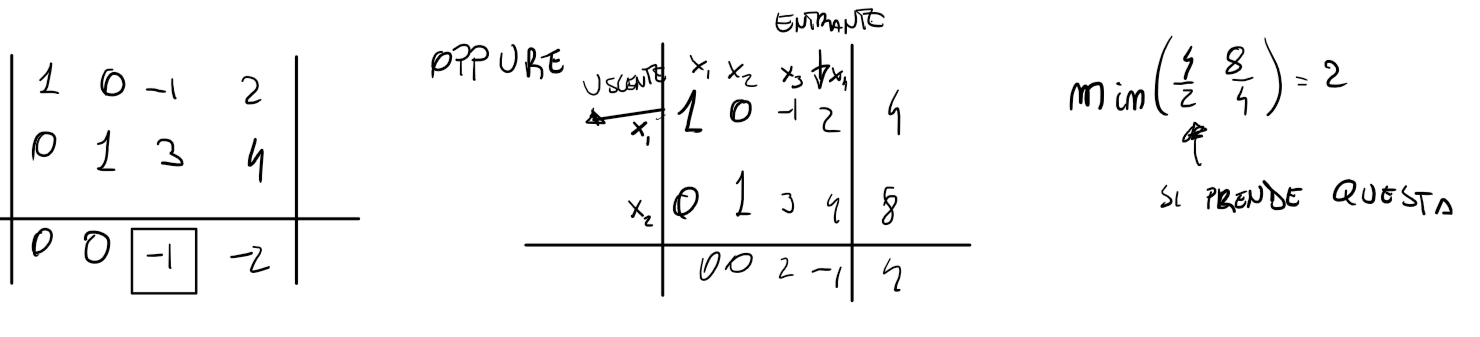
\includegraphics[width=0.5\linewidth]{Images//esempio_simplesso/regola_di_bland.png}
\end{figure}

Per il \textbf{teorema di unicità della soluzione}, abbiamo che se
\[r^T_N=c^T_N-c^T_B B^{-1}N >0\]

allora la soluzione di base $x^T = (B^{-1}b,0)$ è l'unica soluzione ottima del problema.

Se ci sono costi ridotti fuori base che valgono zero, si può forzare il metodo con un'altra iterazione nella quale entra in base la variabile con costo ridotto nullo. In tal caso potremmo scoprire che abbiamo una soluzione ottima oppure che abbiamo un'ulteriore vertice ottimo e, dunque, saranno ottime tutte le loro combinazioni convesse, cioè il segmento che li unisce.

\textbf{Osservazione}\\
Se la colonna con costo ridotto fuori base nullo (riferito al costo finale) ha tutti gli elementi $\leq$ 0 allora esiste un solo vertice ottimo (quello appena trovato) e sono ottime anche tutte le soluzioni sulla semi-retta che esce dal vertice. Pertanto, il poliedro non è limitato e ci sono infinite soluzioni ottime.


\section{Complessità dell'algoritmo del simplesso}
Consideriamo un problema con m vincoli e n variabili. Le attività più dispendiose sono quelle relative all'inversione della matrice di base, dal calcolo del prodotto matriciale $B^{-1}N$ e dei coefficienti di costo ridotto $r^T_N=c^T_N-c^T_B B^{-1}N$. Questi, nel caso peggiore, hanno complessità $O(m^2)$, $O(mn)$ e $O(mn)$. Poiché $m<n$ per ciascuna iterazione la complessità è $O(mn)$. Tuttavia, le iterazione crescono esponenzialmente in base al numero di vertici visitati e, quindi, in base a m e n. Studi hanno dimostrato che, in realtà, crescono solo in base al numero di vincoli m.


\section{Metodo delle due fasi}
Gli esempi considerati hanno sempre avuto solo vincoli di minore uguale. Ma andiamo a vedere cosa succedere in caso di vincoli di maggiore uguale.
\[min(x_1+x_2) \quad  x_1+2x_2\leq3      \quad2x_1+3x_2 \geq 4 \quad   x_1,x_2 \geq 0\]
Questo problema, in forma normale, diventa:
\[min(x_1+x_2) \quad  x_1+2x_2+x_3=3      \quad 2x_1+3x_2-x_4=4 \quad   x_1,x_2,x_3,x_4\geq 0\]
In questo caso la matrice di associata a questo sistema lineare non trova più una base canonica, bensì avremo un vettore $(1,0)$ e un altro $(0,-1)$ e ciò è chiaramente un problema poiché se moltiplicassimo per meno uno, avremmo un -4 come termine noto e ciò non andrebbe più bene perché non sarebbe in forma canonica.

In nostro aiuto arriva il metodo a due fasi per cui, quello che faremo sarà risolvere un problema artificiale per ottenere una soluzione ammissibile di base per avviare il metodo del simplesso.

\section{Fase 1}
La prima fase del metodo del simplesso cerca di risolvere un problema associato al problema iniziale detto \textbf{problema artificiale}. Questo problema non farà altro che trasformare i vincoli $Ax=b\xrightarrow{}Ax+Iy=b$, cioè, aggiungiamo una variabile detta \textbf{variabile artificiale} ad ogni vincolo con il maggiore uguale.
Questa operazione genererà una soluzione del tipo $(x',y')$ dove, però, vorremmo che $\sum_{i=1}^m y_i$ sia minimo (idealmente zero). Così facendo, arrivando ad una soluzione del tipo $(x',0)$ avremmo una soluzione ammissibile di base per il problema iniziale.
\begin{figure}[H]
    \centering
    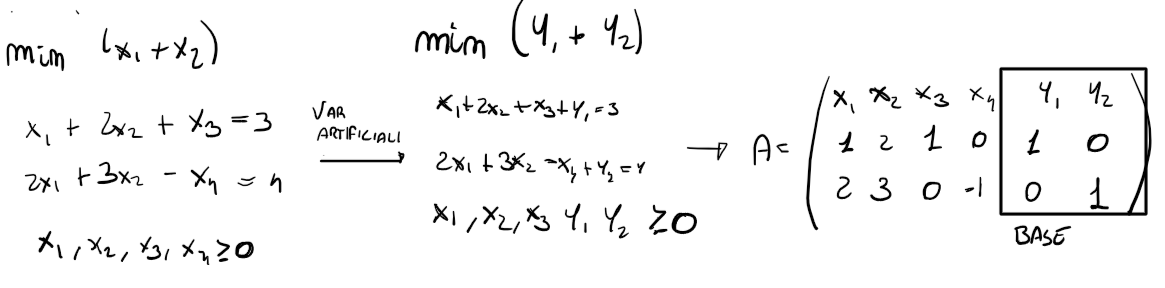
\includegraphics[width=0.7\linewidth]{Images//esempio_simplesso/aggiunta_di_variabili_artificiali.png}
\end{figure} 
Notiamo che abbiamo già la colonna $(1,0)$ per cui, in realtà non avrebbe molto senso aggiungere $y_1$, perciò potremmo lasciare solo la seconda riga. Arrivando a
\[min(y_2)\quad x_1+2x_2+x_3=3 \quad 2x_1+3x_2-x_4+y_2=4 \quad x_1,x_2,x_3,y_2 \geq 0\]

A questo punto, appena trovata la soluzione della funzione obiettivo del problema artificiale $z'=\sum_{i-1}^my'$, possiamo avere due situazioni:
\begin{enumerate}
    \item $z'>0$: questo accade perché abbiamo un qualche $y'$ positivo e, dunque, non ci sono soluzioni $Ax+Iy = b$ che sono soluzioni anche di $Ax=b$. Ciò vuol dire che il problema di base non è ammissibile poiché potrebbero esserci dei vincoli in contraddizione o incompatibili.
    \item $z'=0$ Siamo riusciti ad avere tutti gli $y' = 0$ e, dunque, il problema iniziale ha soluzione di base ammissibile il vertice che abbiamo trovato $x'$ nel problema artificiale. 
\end{enumerate}
\section{Fase 2}
Si risolve il problema utilizzando la tabella del simplesso finale della fase 1 aggiornando la riga dei costi ridotti in funzione della funzione obiettivo del problema originale. Se le variabili artificiali non fanno parte della base, allora si possono eliminare e si semplifica la tabella. 
Se alcune variabili artificiali sono in base, allora rimangono lì anche nella fase 2.  Il metodo procede cercando di far uscire dalla base le variabili artificiali. Se non si riesce per qualunque motivo, allora ci sono dei vincoli ridondanti che coinvolgono le variabili artificiali che si devono eliminare. Per cui, andremo a eliminare la riga corrispondente (che rappresenta il vincolo ridondante) e la colonna della variabile artificiale riducendo la dimensione del problema.

\section{Esempio Metodo a Due Fasi}
Supponiamo di avere il seguente problema, che trasformiamo in forma standard:
\begin{figure}[H]
    \centering
    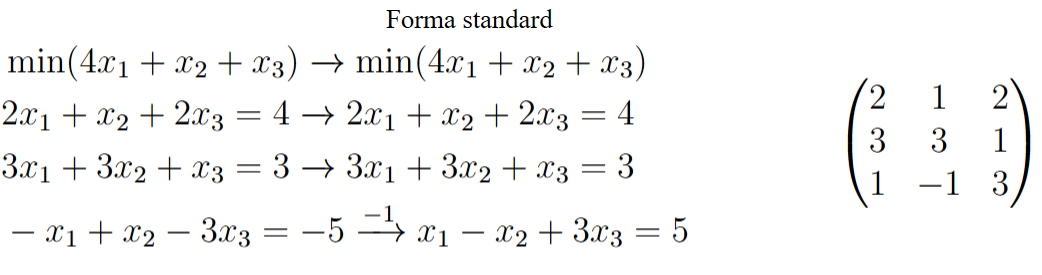
\includegraphics[width=0.7\linewidth]{Images/esempio_due_fasi/problema_iniziale.png}
\end{figure}
Da questo, non potendo ricavare una base iniziale da cui partire, passiamo al problema artificiale:
\begin{figure}[H]
    \centering
    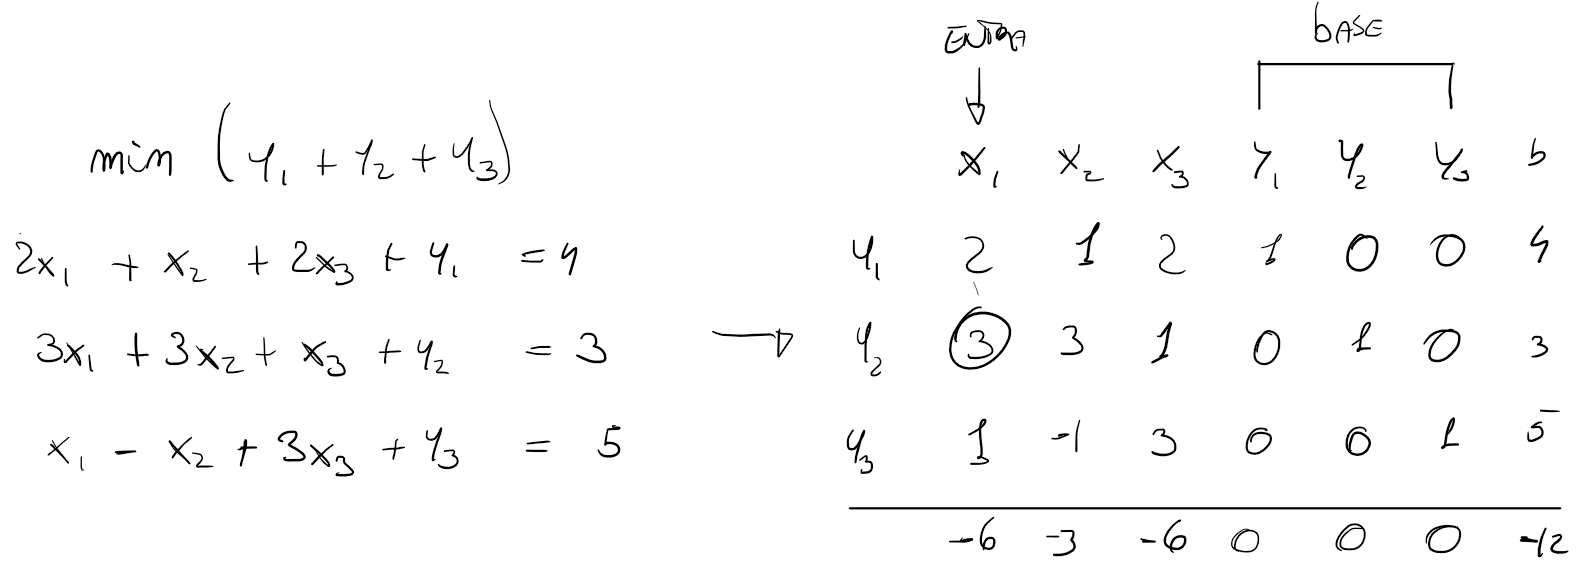
\includegraphics[width=0.7\linewidth]{Images/esempio_due_fasi/problema_artificiale.png}
\end{figure}
La cui riga dei costi ridotti è calcolata:
\[r_i = \text{variabile sopra in f.o.}-(\text{variabili in base in f.o.}) \times (\text{vettore colonna i})\]
Dove la moltiplicazione sarà una moltiplicazione riga per colonna. 

Continuiamo come sempre con il metodo del simplesso e, dopo alcuni passaggi, arriveremo in questa situazione.
\begin{figure}[H]
    \centering
    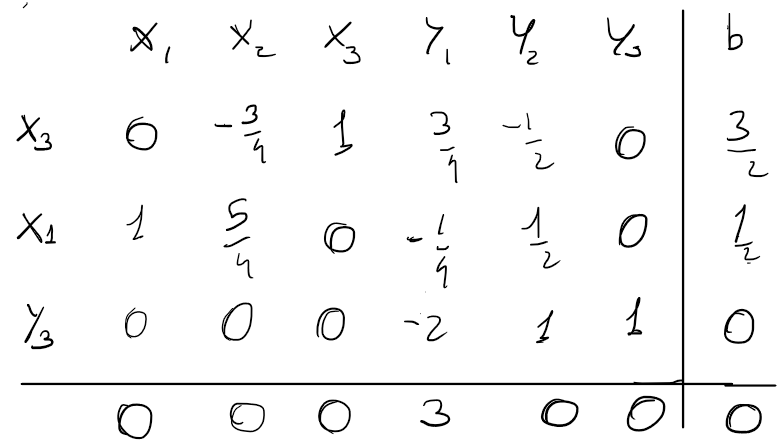
\includegraphics[width=0.5\linewidth]{Images/esempio_due_fasi/risultato_problema_artificiale.png}
\end{figure}
Una volta notato come il risultato della funzione obiettivo sia 0, vuol dire che abbiamo una soluzione ammissibile e possiamo continuare con la seconda fase. Ricalcolando\footnote{Utilizzando la stessa formula di prima} il valore della funzione obiettivo ed eliminando le colonne superflue $y_1, y_2$ che si trovano fuori base.
\begin{figure}[H]
    \centering
    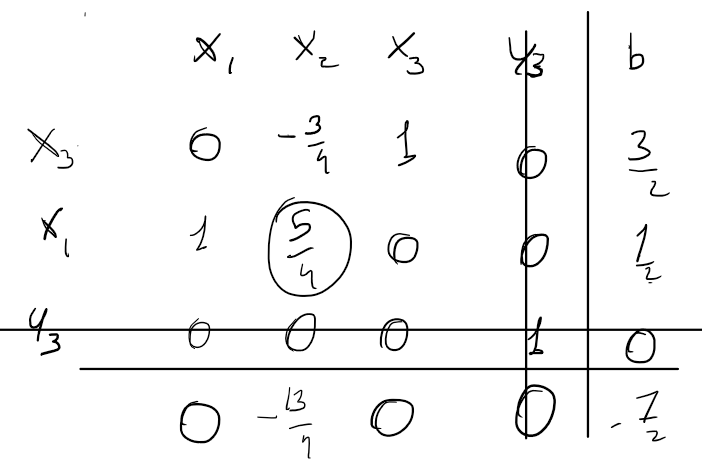
\includegraphics[width=0.4\linewidth]{Images/esempio_due_fasi/fase_2.png}
\end{figure}
Notiamo inoltre che $y_3$ in questo sistema vale 0, per cui possiamo anche tagliare la sua riga e la colonna associata dato che questa si trovava momentaneamente in base. Procedendo con il classico metodo del simplesso arriveremo alla seguente soluzione:
\begin{figure}[H]
    \centering
    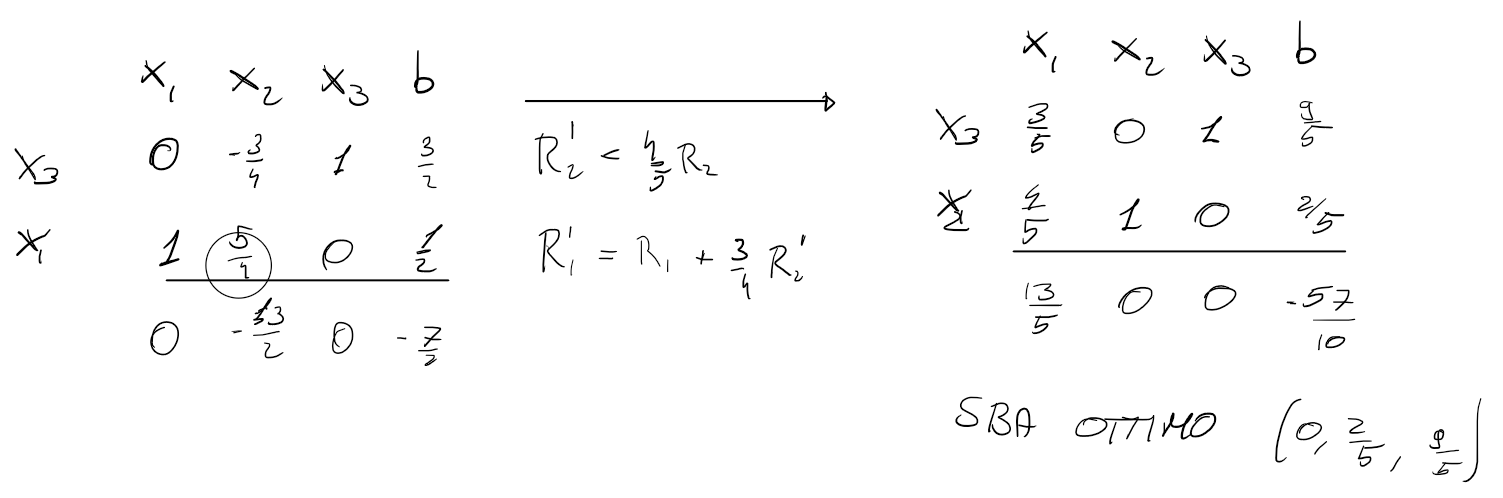
\includegraphics[width=0.9\linewidth]{Images/esempio_due_fasi/soluzione.png}
\end{figure}

